%%%%%%%%%%%%%%%%%%%%%%%%%%%%%%%%%%%%%%%%%%%%%%%%%%%%%%%%%%%%
%%  Class 1, NE 155
%%

\documentclass[xcolor=x11names,compress]{beamer}

\definecolor{CoolBlack}{rgb}{0.0, 0.18, 0.39}
%% General document %%%%%%%%%%%%%%%%%%%%%%%%%%%%%%%%%%
\usepackage{graphicx}
\usepackage{tikz}
\usetikzlibrary{decorations.fractals}
\usepackage{hyperref}
%%%%%%%%%%%%%%%%%%%%%%%%%%%%%%%%%%%%%%%%%%%%%%%%%%%%%%

%% Beamer Layout %%%%%%%%%%%%%%%%%%%%%%%%%%%%%%%%%%
\useoutertheme[subsection=false,shadow]{miniframes}
\useinnertheme{default}
\usefonttheme{serif}
\usepackage{palatino}
\usepackage{tabu}
% Links
\usepackage{hyperref}
\definecolor{links}{HTML}{003262}
\hypersetup{colorlinks,linkcolor=,urlcolor=links}

% addition of color
\usepackage{xcolor}
\definecolor{CoolBlack}{rgb}{0.0, 0.18, 0.39}
\definecolor{byellow}{rgb}{0.55037, 0.38821, 0.06142}
\definecolor{dgreen}{rgb}{0.,0.6,0.}
\definecolor{RawSienna}{cmyk}{0,0.72,1,0.45}
\definecolor{forestgreen(web)}{rgb}{0.13, 0.55, 0.13}
\definecolor{cardinal}{rgb}{0.77, 0.12, 0.23}

\setbeamerfont{title like}{shape=\scshape}
\setbeamerfont{frametitle}{shape=\scshape}

\setbeamercolor*{lower separation line head}{bg=CoolBlack}
\setbeamercolor*{normal text}{fg=black,bg=white}
\setbeamercolor*{alerted text}{fg=dgreen} % just testing; I think this looks better
\setbeamercolor*{example text}{fg=black}
\setbeamercolor*{structure}{fg=black}

\setbeamercolor*{palette tertiary}{fg=black,bg=black!10}
\setbeamercolor*{palette quaternary}{fg=black,bg=black!10}

% Margins
\usepackage{changepage}

\mode<presentation>
{
  \definecolor{berkeleyblue}{HTML}{003262}
  \definecolor{berkeleygold}{HTML}{FDB515}
  \usetheme{Boadilla}      % or try Darmstadt, Madrid, Warsaw, Boadilla...
  %\usecolortheme{dove} % or try albatross, beaver, crane, ...
  \setbeamercolor{structure}{fg=berkeleyblue,bg=berkeleygold}
  \setbeamercolor{palette primary}{bg=berkeleyblue,fg=white} % changed this
  \setbeamercolor{palette secondary}{fg=berkeleyblue,bg=berkeleygold} % changed this
  \setbeamercolor{palette tertiary}{bg=berkeleyblue,fg=white} % changed this
  \usefonttheme{structurebold}  % or try serif, structurebold, ...
  \useinnertheme{circles}
  \setbeamertemplate{navigation symbols}{}
  \setbeamertemplate{caption}[numbered]
  \usebackgroundtemplate{}
}
%---

\renewcommand{\(}{\begin{columns}}
\renewcommand{\)}{\end{columns}}
\newcommand{\<}[1]{\begin{column}{#1}}
\renewcommand{\>}{\end{column}}

% adding slide numbers
\addtobeamertemplate{navigation symbols}{}{%
    \usebeamerfont{footline}%
    \usebeamercolor[fg]{footline}%
    \hspace{1em}%
    \insertframenumber/\inserttotalframenumber
}

% equation stuff
\newcommand{\Macro}{\ensuremath{\Sigma}}
\newcommand{\Sn}{\ensuremath{S_N} }
\newcommand{\vOmega}{\ensuremath{\hat{\Omega}}}
\usepackage{mathrsfs}
\usepackage[mathcal]{euscript}
\usepackage{amssymb}
\usepackage{amsthm}
\usepackage{epsfig}
\usepackage{amsmath}
%%%%%%%%%%%%%%%%%%%%%%%%%%%%%%%%%%%%%%%%%%%%%%%%%%
% title stuff for footer
\title{NE 155}
\author{R.\ N.\ Slaybaugh}
\date{April 15, 2015}

\begin{document}

%%%%%%%%%%%%%%%%%%%%%%%%%%%%%%%%%%%%%%%%%%%%%%%%%%%%%%
%%%%%%%%%%%%%%%%%%%%%%%%%%%%%%%%%%%%%%%%%%%%%%%%%%%%%%
\begin{frame}
\title{NE 155\\Introduction to Numerical Simulations in Radiation Transport}
\subtitle{Lecture 33: Probability and Statics}
\titlepage
\end{frame}

%%%%%%%%%%%%%%%%%%%%%%%%%%%%%%%%%%%%%%%%%%%%%%%%%%%%%%
%%%%%%%%%%%%%%%%%%%%%%%%%%%%%%%%%%%%%%%%%%%%%%%%%%%%%%
\begin{frame}{Major Components of MC Algorithm}

\begin{itemize}
  \item \textbf{PDFs}: the physical/mathematical system must be described by a set of pdfs.
  % That's next class
  \pause
  \item \textbf{Random number generator}: a source of random \#s uniformly distributed on the unit interval.
  % We're going to skip this
  \pause
  \item \textbf{Sampling rule}: prescription for sampling the pdf (given having random \#s)
  % That's also next class
  \pause
  \item \textbf{Scoring}: the outcomes must be accumulated/\underline{tallied} for quantities of interest
  % we might cover it
  \pause
  \item \textit{\textbf{Error estimation}: an estimate of the statistical error (\underline{variance}) of the solution}
  % This class!
    \pause
  \item \textbf{Variance Reduction}: methods for reducing the variance and computation time simultaneously
  % briefly this class, maybe more at the end
    \pause
  \item \textbf{Parallelization}: efficient use of computers
  % probably not
\end{itemize}
\end{frame}

%%%%%%%%%%%%%%%%%%%%%%%%%%%%%%%%%%%%%%%%%%%%%%%%%%%%%%
%%%%%%%%%%%%%%%%%%%%%%%%%%%%%%%%%%%%%%%%%%%%%%%%%%%%%%
\begin{frame}{Outline / Learning Objectives}

\begin{columns}
  \begin{column}{0.5\textwidth}
    \begin{enumerate}
    \item Probability Density Functions
    \item Standard Statistical Quantities
    \item Accuracy vs.\ Precision
    \item Central Limit Theorem
    \item Relative Error
    \end{enumerate}
  \end{column}
  \begin{column}{0.5\textwidth}
    \begin{enumerate}
    \item Understand the derivation of basic statistical quantities
    \item Be able to explain the difference between accuracy and precision 
    \item Understand how to interpret and apply confidence intervals
    \item Understand derivation and use of relative error
    \end{enumerate}
  \end{column}
\end{columns}

\vspace*{1em}
Notes derived from Jasmina Vujic and Paul Wilson
\end{frame}


%%%%%%%%%%%%%%%%%%%%%%%%%%%%%%%%%%%%%%%%%%%%%%%%%%%%%%
%%%%%%%%%%%%%%%%%%%%%%%%%%%%%%%%%%%%%%%%%%%%%%%%%%%%%%
\begin{frame}{Fundamental Concept}

\begin{itemize}
  \item Many individual particle histories are simulated
  \item Each physical event is determined by
randomly sampling a \alert{probability distribution}
  \item Each history can contribute to the physical
measurement of interest
    \begin{itemize}
    \item $x_i$ = contribution of history $i$
    \item Different ways to calculate score
      \begin{itemize}
      \item Does particle cross surface?
      \item How much time does particle spend in particular region?
      \end{itemize}
    \end{itemize}
\end{itemize}
\end{frame}


%%%%%%%%%%%%%%%%%%%%%%%%%%%%%%%%%%%%%%%%%%%%%%%%%%%%%%
%%%%%%%%%%%%%%%%%%%%%%%%%%%%%%%%%%%%%%%%%%%%%%%%%%%%%%
\begin{frame}{Fundamental Concept}

\begin{itemize}
  \item Set of individual contributions, ${x_i}$,
forms a \textit{probability distribution}
\end{itemize}
  	\begin{figure}
  	\begin{center}
  		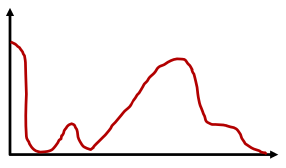
\includegraphics[height=1in,clip]{pdf}
	\end{center}
  	\end{figure}

\begin{itemize}
  \item We are interested in the mean value of that contribution, $\overline{x_i}$, and its variance, $S_{\overline{x}}^2$
\end{itemize}

\end{frame}


%%%%%%%%%%%%%%%%%%%%%%%%%%%%%%%%%%%%%%%%%%%%%%%%%%%%%%
%%%%%%%%%%%%%%%%%%%%%%%%%%%%%%%%%%%%%%%%%%%%%%%%%%%%%%
\begin{frame}{Two Encounters with Probability Distributions}

\begin{itemize}
    \item Probability distributions for the outcome
of each physical event
    \item We use \textbf{Random Sampling} techniques to
evaluate these at each occurrence
    \item Underlying probability distribution for
each physical measurement of interest
    \item We estimate the statistical moments of
these distributions to get our physical
answers
\end{itemize}
\end{frame}


%%%%%%%%%%%%%%%%%%%%%%%%%%%%%%%%%%%%%%%%%%%%%%%%%%%%%%
%%%%%%%%%%%%%%%%%%%%%%%%%%%%%%%%%%%%%%%%%%%%%%%%%%%%%%
\begin{frame}{To the Board}

  	\begin{figure}
  	\begin{center}
  		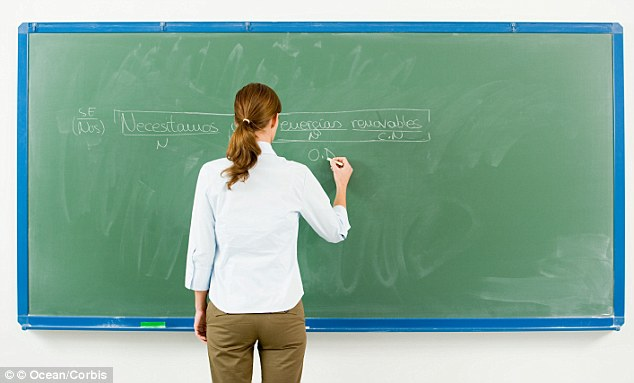
\includegraphics[height=2in,clip]{board}
  		%http://topicalteaching.com/2013/09/08/how-should-teachers-dress/
	\end{center}
  	\end{figure}

\end{frame}


%%%%%%%%%%%%%%%%%%%%%%%%%%%%%%%%%%%%%%%%%%%%%%%%%%%%%%
%%%%%%%%%%%%%%%%%%%%%%%%%%%%%%%%%%%%%%%%%%%%%%%%%%%%%%
\begin{frame}{Two Types of MC Methodology}

\alert{Analog}
\begin{itemize}
    \item Natural laws are \textbf{preserved}
    \item The game is the ``analog" of the physical problem of interest (the history of each particle is simulated exactly)
\end{itemize}
\pause

\alert{Non-Analog}
\begin{itemize}
    \item To reduce computation time, the strict analog simulation of particles is abandoned (i.e.\ we CHEAT)
    \item Variance Reduction techniques:
    \begin{itemize}
    \item Absorption suppression
    \item Russian Roulette (history termination)
    \item Splitting (history propagation)
    \item Forced collisions
    \item Source biasing
    \item Hybrid methods
    \end{itemize}
    \end{itemize}

\end{frame}


%%%%%%%%%%%%%%%%%%%%%%%%%%%%%%%%%%%%%%%%%%%%%%%%%%%%%%
%%%%%%%%%%%%%%%%%%%%%%%%%%%%%%%%%%%%%%%%%%%%%%%%%%%%%%
\begin{frame}{Analog vs.\ Weighted MC}

\alert{Analog}
\begin{itemize}
    \item No alteration of PDFs
    \item At collision, particle is killed if absorption
    \item Particle is born with weight 1
    \item weight unchanged throughout history
    \item Score when tallying events is 1
\end{itemize}
\pause

\alert{Non-Analog} (weighted)
\begin{itemize}
    \item Alter PDFs to favor events of interest
    \item Particle can have different birth weight
    \item Weight is altered if biased PDF is used
    \item Particle survives ``absorption" and weight is changed
    \item Splitting and RR can change weight
    \item Score current weight when tallying
    \end{itemize}

\end{frame}


%%%%%%%%%%%%%%%%%%%%%%%%%%%%%%%%%%%%%%%%%%%%%%%%%%%%%%
%%%%%%%%%%%%%%%%%%%%%%%%%%%%%%%%%%%%%%%%%%%%%%%%%%%%%%
\begin{frame}{Probability \& Statistics Summary}

    \begin{itemize}
    \item Rich variety of statistical analysis is
possible.
\pause
\vspace*{.5em}
    \item The difference between accuracy and
precision is important
\pause
\vspace*{.5em}
    \item Accuracy is not always known and can
be difficult to improve
\pause
\vspace*{.5em}
    \item Precision can be improved by more
histories in a measurement, but not
always more histories in a problem
    \end{itemize}

\end{frame}


\end{document}
